\documentclass[11pt,a4paper]{article}

\usepackage[utf8]{inputenc}
\usepackage[spanish,es-nodecimaldot]{babel}
\usepackage[T1]{fontenc}
\usepackage{lmodern}
\usepackage{geometry}
\geometry{top=2.5cm, bottom=2.5cm, left=2.5cm, right=2.5cm}

\usepackage{amsmath,amssymb}
\usepackage{graphicx}
\usepackage{booktabs}
\usepackage{float}
\usepackage{hyperref}
\hypersetup{colorlinks=true, linkcolor=black, urlcolor=blue}

\setlength{\parindent}{0pt}
\setlength{\parskip}{6pt}

\title{
    \vspace{-1.2cm}
    \textbf{Sistemas de Control}\\
    \large Trabajo de Laboratorio Integrador: Desarrollo de controlador atraso-adelanto
}
\author{Tomás Gómez Pizarro \quad\and\quad Mikael Rodríguez}
\date{Noviembre 2026}

\begin{document}

\maketitle

La planta es la misma del laboratorio anterior:
\begin{equation}
    G(s) = \frac{1}{(0{,}01s + 1)(0{,}0047s + 1)} = \frac{21276{,}6}{(s + 100)(s + 212{,}77)}
\end{equation}
con realimentación unitaria. Las especificaciones para el lazo cerrado son:
\begin{itemize}
    \item $PO \le 5\%$
    \item $T_s \le 0{,}02\text{ s}$ (criterio del $2\%$)
    \item $e_{ss} \le 0{,}06$ ante un escalón unitario
\end{itemize}

Todos los cálculos y figuras se obtienen con el Live Script \texttt{TP\_Lab3.mlx}.

\section*{Punto 1. Diseño del compensador de adelanto}

El compensador tiene la forma
\begin{equation}
    G_c(s) = K_a \, \frac{s + z_l}{s + p_l}, \qquad z_l < p_l
\end{equation}
donde $K_a = 1 + R_7/R_9$ es la ganancia de la etapa no inversora. El diseño se hace en forma analítica con las condiciones de ángulo y módulo.

\subsection*{Región admisible y punto de diseño $s_d$}

Las especificaciones de $PO$ y $T_s$ delimitan una región del plano $s$:
\begin{equation}
    PO \le 5\% \implies \zeta \ge \frac{-\ln(0{,}05)}{\sqrt{\pi^2 + \ln^2(0{,}05)}} = 0{,}690
    \qquad\qquad
    T_s \approx \frac{4}{\sigma} \le 0{,}02 \implies \sigma \ge 200\ \text{s}^{-1}
\end{equation}

No se toma $s_d$ en el vértice de la región ($\zeta = 0{,}69$, $\sigma = 200$) porque $T_s \approx 4/\sigma$ es una aproximación: simulando ese punto el tiempo de establecimiento da $\approx 20{,}7$ ms. Además los componentes reales tienen tolerancia. Por eso se deja un margen y se elige:
\begin{equation}
    \zeta_d = 0{,}72,\quad \sigma_d = 230\ \text{s}^{-1}
    \implies s_d = -230 \pm j\,221{,}7, \quad \omega_n = 319{,}4\ \text{rad/s}
\end{equation}
que corresponde a $PO = 3{,}84\%$ y $T_s \approx 17{,}4$ ms.

\subsection*{Condición de ángulo}

La fase de la planta en $s_d$ es
\begin{equation}
    \angle G(s_d) = -\angle(s_d + 100) - \angle(s_d + 212{,}77) = -120{,}39^\circ - 94{,}45^\circ = -214{,}83^\circ
\end{equation}
Para que $s_d$ pertenezca al lugar de raíces la fase total debe ser $-180^\circ$, por lo que el compensador debe aportar
\begin{equation}
    \phi = -180^\circ + 214{,}83^\circ = 34{,}83^\circ
\end{equation}

\textbf{Cero.} Se ubica sobre el polo rápido de la planta, $z_l = 212{,}77$, para cancelarlo. Así el lazo queda de segundo orden y las fórmulas de $PO$ y $T_s$ se aplican sin polos adicionales. Cancelar el polo en $-100$ también es posible, pero da una constante de error menor ($K_p = 0{,}94$ contra $1{,}835$ para el mismo $s_d$), lo que complica el punto siguiente. En la práctica la cancelación no es exacta y queda un par polo-cero cercano, cuyo efecto en la respuesta es chico.

\textbf{Polo.} El cero aporta $\angle(s_d + z_l) = 94{,}45^\circ$, de modo que el polo debe aportar $94{,}45^\circ - 34{,}83^\circ = 59{,}61^\circ$:
\begin{equation}
    p_l = \sigma_d + \frac{\omega_d}{\tan(59{,}61^\circ)} = 230 + \frac{221{,}7}{1{,}706} = 360\ \text{s}^{-1}
\end{equation}
Como control, con la cancelación el lazo es $K/[(s+100)(s+p_l)]$ y la parte real de los polos complejos es el promedio de los polos, $\sigma_d = (100 + p_l)/2$, que da también $p_l = 360$.

\subsection*{Condición de módulo}

Con $z_l$ y $p_l$ fijados, $K_a$ se obtiene de $|G_c(s_d)\,G(s_d)| = 1$:
\begin{equation}
    K_a = \frac{1}{\left|\dfrac{s_d + z_l}{s_d + p_l}\, G(s_d)\right|} = 3{,}104
\end{equation}
El compensador resultante es
\begin{equation}
    G_c(s) = 3{,}104\,\frac{s + 212{,}77}{s + 360}
\end{equation}
con polos de lazo cerrado en $-230 \pm j\,221{,}7$ y $-212{,}77$ (cancelado por el cero). Como $K_a > 1$, es realizable con la etapa no inversora. La Figura~\ref{fig:punto1_lgr} muestra el lugar de raíces del sistema compensado pasando por $s_d$.

\begin{figure}[H]
    \centering
    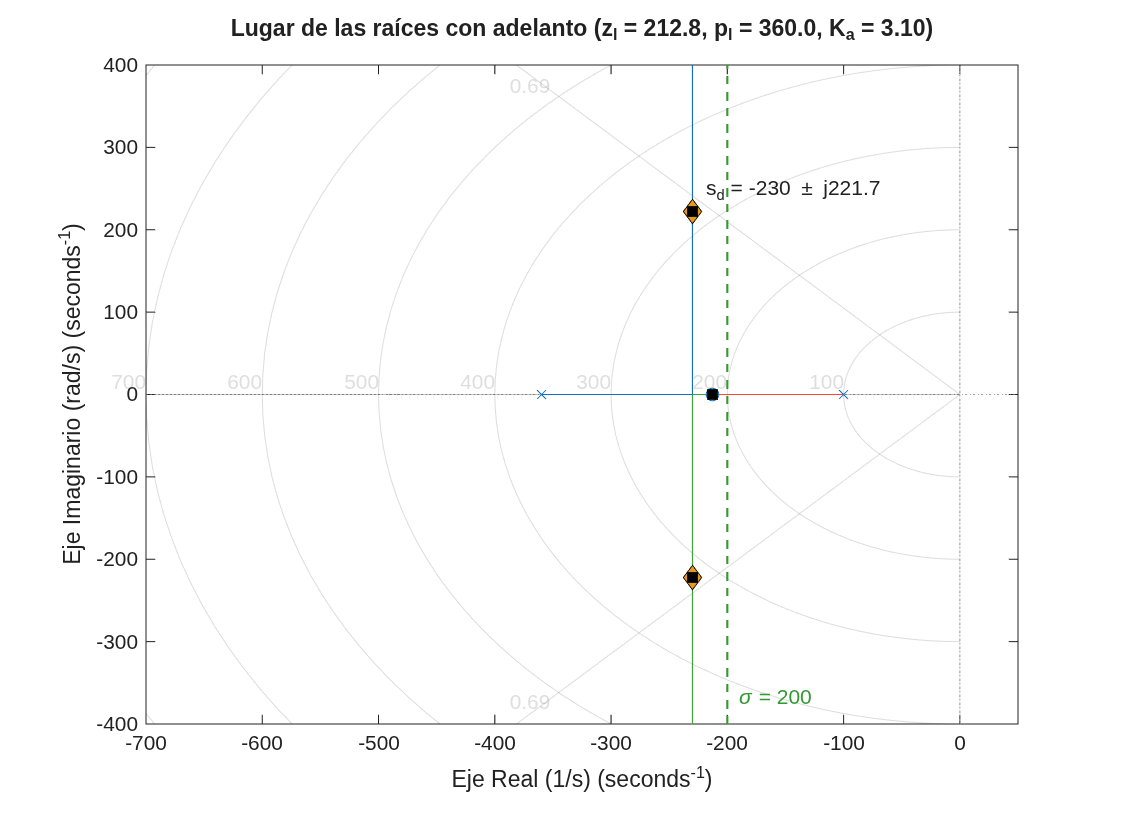
\includegraphics[width=0.78\textwidth]{figuras/punto1_lgr_adelanto.png}
    \caption{Lugar de raíces de $\frac{s+z_l}{s+p_l}G(s)$ con la cota $\zeta = 0{,}69$ y la recta $\sigma = 200$. Rombo: $s_d$; cuadrados: polos de lazo cerrado con $K_a = 3{,}104$.}
    \label{fig:punto1_lgr}
\end{figure}

\textbf{Sobre el error estacionario.} Con el adelanto la constante de error es $K_p = K_a\, z_l/p_l = 1{,}835$, lejos de la necesaria $K_p \ge 15{,}67$. En teoría se podría cumplir $e_{ss}$ solo con el adelanto eligiendo un $s_d$ mucho más a la izquierda: manteniendo $\zeta = 0{,}72$ y la cancelación, recién con $p_l \approx 3300$ ($\sigma \approx 1700$) se llega a $K_p \approx 15{,}9$, pero eso requiere $K_a \approx 247$. Esto no es viable en la práctica: una ganancia tan grande lleva a los amplificadores a saturación ($\pm 8{,}5$ V), y el modelo lineal con el que se diseñó deja de valer. Por eso el adelanto se usa solo para el transitorio y el error se corrige con un compensador de atraso.

\section*{Punto 2. Respuesta al escalón con el compensador de adelanto}

La Figura~\ref{fig:punto2_escalon} muestra la respuesta al escalón unitario del sistema $T(s) = \dfrac{G_c G}{1 + G_c G}$.

\begin{figure}[H]
    \centering
    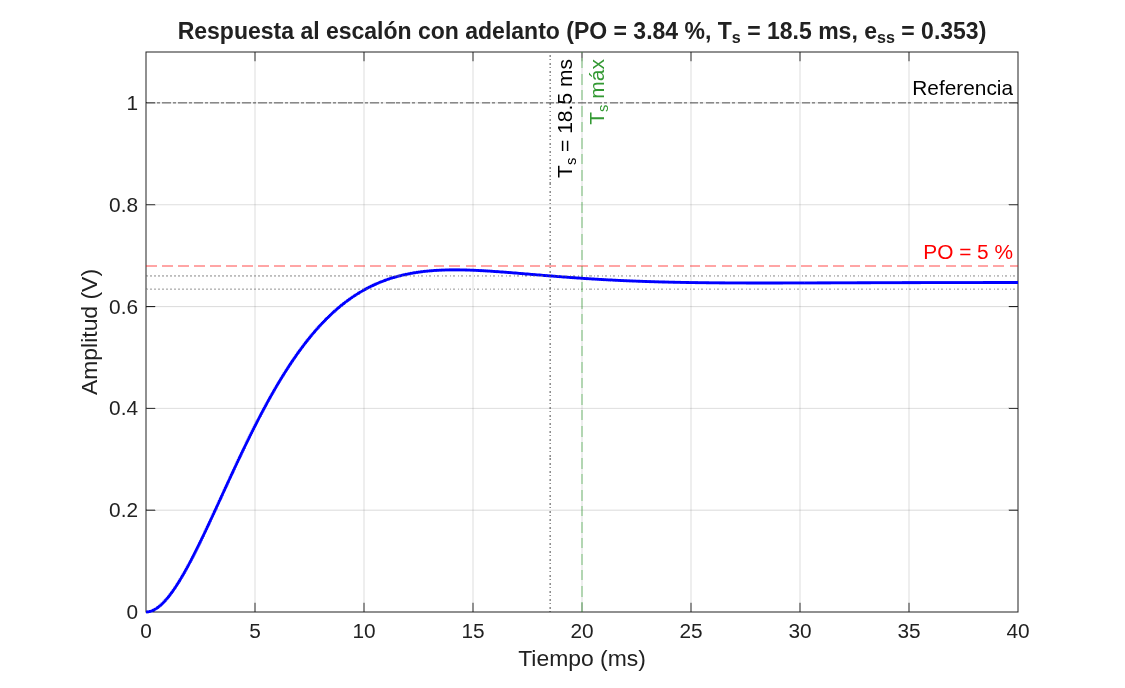
\includegraphics[width=0.78\textwidth]{figuras/punto2_escalon_adelanto.png}
    \caption{Respuesta al escalón unitario con el compensador de adelanto. Líneas punteadas: banda del $2\%$ y cota de $PO$.}
    \label{fig:punto2_escalon}
\end{figure}

\begin{table}[H]
    \centering
    \caption{Desempeño con el compensador de adelanto.}
    \vspace{2mm}
    \begin{tabular}{lccc}
        \toprule
        \textbf{Métrica} & \textbf{Requerido} & \textbf{Obtenido} & \textbf{Cumple} \\
        \midrule
        Sobrepaso ($PO$) & $\le 5\%$ & $3{,}84\%$ & Sí \\
        Tiempo de establecimiento ($T_s$) & $\le 20$ ms & $18{,}5$ ms & Sí \\
        Error estacionario ($e_{ss}$) & $\le 0{,}06$ & $0{,}353$ & No \\
        \bottomrule
    \end{tabular}
    \label{tab:punto2}
\end{table}

El $PO$ coincide con el de diseño porque, con la cancelación, el sistema es de segundo orden. El $T_s$ simulado ($18{,}5$ ms) es algo mayor que la estimación $4/\sigma_d = 17{,}4$ ms, pero sigue dentro de la especificación gracias al margen elegido en $s_d$.

El error estacionario no se cumple. El sistema es de tipo 0 y
\begin{equation}
    e_{ss} = \frac{1}{1 + K_p} = \frac{1}{1 + 1{,}835} = 0{,}353
\end{equation}
es decir, la salida se estabiliza en $0{,}647$ V. Para llegar a $e_{ss} \le 0{,}06$ hay que multiplicar $K_p$ por al menos $15{,}67/1{,}835 \approx 8{,}5$, que es lo que se resuelve con el compensador de atraso en el punto siguiente.

\section*{Punto 3. Diseño del compensador de atraso}

El compensador de atraso tiene la forma
\begin{equation}
    G_{ca}(s) = \frac{s + z_a}{s + p_a}, \qquad z_a > p_a
\end{equation}
En continua aporta una ganancia $G_{ca}(0) = z_a/p_a = \alpha$, mientras que para frecuencias altas frente a $z_a$ su ganancia es aproximadamente 1.

\subsection*{a. Relación $\alpha$}

La constante de error del sistema con ambos compensadores es $K_p = \alpha \cdot 1{,}835$. Para $e_{ss} \le 0{,}06$:
\begin{equation}
    e_{ss} = \frac{1}{1 + K_p} \le 0{,}06 \implies K_p \ge 15{,}67 \implies \alpha \ge \frac{15{,}67}{1{,}835} = 8{,}54
\end{equation}
Con $\alpha = 10$ el error quedaría en $0{,}052$, cerca del límite. Para dejar margen frente a las tolerancias de los componentes se elige
\begin{equation}
    \alpha = 12 \implies K_p = 22{,}0, \quad e_{ss} = 0{,}0435
\end{equation}

\subsection*{b. Ubicación del cero y el polo}

Si se ubican el cero y el polo cerca del origen, por ejemplo $z_a = \sigma_d/10 = 23$ y $p_a = 1{,}92$, de modo que vistos desde $s_d$ aporten casi el mismo ángulo y no muevan los polos dominantes. Con esta elección los polos dominantes casi no cambian, pero aparece un polo de lazo cerrado lento en $-16{,}6$. La respuesta sube rápido hasta el valor que tenía con el adelanto solo ($\approx 0{,}65$) y después llega al valor final ($0{,}956$) con la constante de tiempo de ese polo, por lo que $T_s$ pasa a $163$ ms. Como el atraso tiene que llevar la salida de $0{,}65$ a $0{,}96$, esa cola no es chica, y cuanto más cerca del origen se pone $z_a$ más lenta resulta.

Por eso se barrió $z_a$ manteniendo $\alpha = 12$ (Tabla~\ref{tab:barrido}).

\begin{table}[H]
    \centering
    \caption{Barrido de la ubicación del cero del atraso con $\alpha = 12$.}
    \vspace{2mm}
    \begin{tabular}{ccccc}
        \toprule
        $z_a$ & $p_a$ & $PO$ & $T_s$ (ms) & Polo de LC más lento \\
        \midrule
        23 & 1,92 & 0\% & 162,8 & $-16{,}6$ \\
        40 & 3,33 & 0\% & 85,5 & $-30{,}6$ \\
        60 & 5,00 & 0\% & 48,9 & $-49{,}4$ \\
        70 & 5,83 & 0\% & 37,8 & $-60{,}2$ \\
        80 & 6,67 & 0\% & 14,6 & $-72{,}0$ \\
        \textbf{85} & \textbf{7,08} & \textbf{0,69\%} & \textbf{13,5} & $\mathbf{-78{,}4}$ \\
        90 & 7,50 & 2,01\% & 17,6 & $-85{,}2$ \\
        95 & 7,92 & 3,31\% & 21,0 & $-92{,}4$ \\
        110 & 9,17 & 6,98\% & 24,8 & $-116{,}6$ \\
        \bottomrule
    \end{tabular}
    \label{tab:barrido}
\end{table}

Para $z_a$ chico el $T_s$ está dominado por la cola lenta; para $z_a$ grande el atraso deja de estar cerca del origen visto desde $s_d$, resta fase y aumenta el $PO$. Las tres especificaciones se cumplen para $z_a$ entre 80 y 90. Se elige $z_a = 85$, cerca del polo de la planta en $-100$, con lo que el polo de lazo cerrado asociado al atraso ($-78{,}4$) ya no es lento:
\begin{equation}
    G_{ca}(s) = \frac{s + 85}{s + 7{,}08}
\end{equation}
A cambio, el transitorio se modifica respecto del logrado con el adelanto, lo que se ve en el punto siguiente.

Cabe aclarar que esta no es la forma habitual de diseñar el atraso. Normalmente se ubica el cero aproximadamente una década por debajo de los polos dominantes, de modo que no altere el transitorio, y se acepta una cola lenta de poca amplitud. Esto funciona bien cuando el aumento de $K_p$ requerido es moderado. En este caso el $\alpha$ necesario es grande y la cola resulta del orden del $30\%$ del valor final. Como el adelanto se diseñó primero cancelando el polo en $-212{,}77$, el polo de la planta en $-100$ quedó disponible, y ubicar $z_a$ cerca de él fue la forma de cumplir las tres especificaciones sin rediseñar el adelanto.

\section*{Punto 4. Sistema final}

El controlador final es
\begin{equation}
    G_{total}(s) = K_a\, G_{ca}(s)\, \frac{s + z_l}{s + p_l} = 3{,}104\, \frac{(s + 85)(s + 212{,}77)}{(s + 7{,}08)(s + 360)}
\end{equation}
y la función de transferencia a lazo cerrado, simplificando la cancelación en $-212{,}77$, resulta
\begin{equation}
    Sys_c(s) = \frac{G_{total}\, G}{1 + G_{total}\, G} = \frac{66045\,(s + 85)}{(s + 78{,}44)\,(s^2 + 388{,}6\,s + 74820)}
\end{equation}
con polos en $-194{,}3 \pm j\,192{,}5$ ($\zeta = 0{,}71$) y $-78{,}4$, y un cero en $-85$.

\subsection*{a. Respuesta al escalón}

\begin{figure}[H]
    \centering
    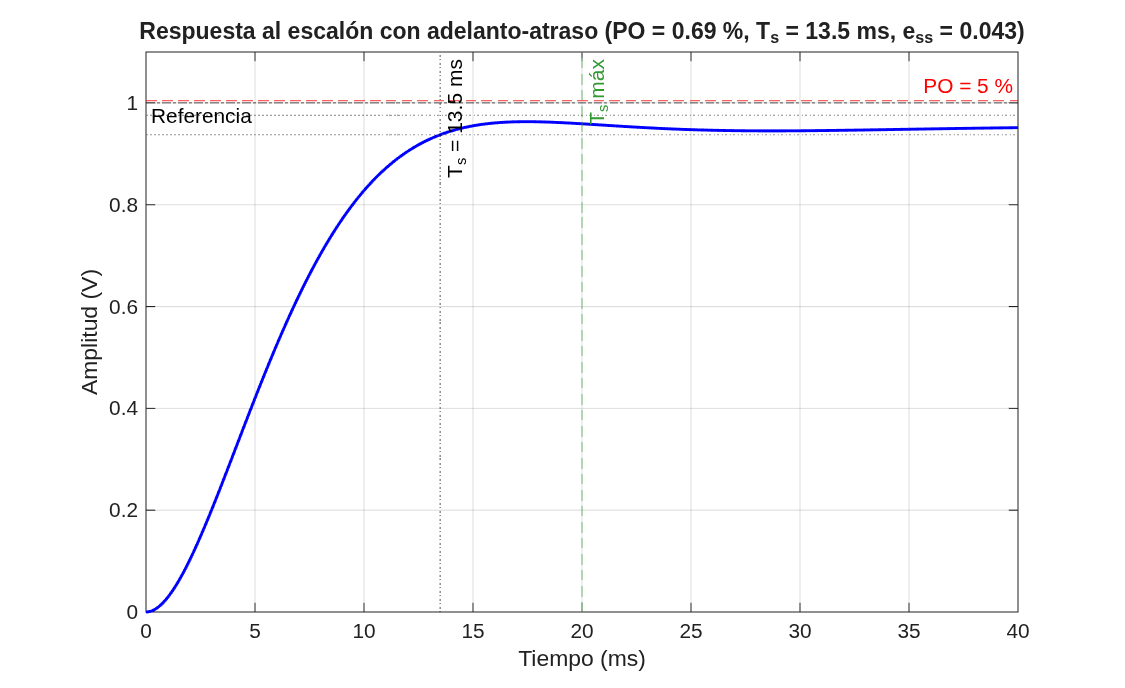
\includegraphics[width=0.78\textwidth]{figuras/punto4_escalon_adelanto_atraso.png}
    \caption{Respuesta al escalón unitario con el compensador de adelanto-atraso.}
    \label{fig:punto4_escalon}
\end{figure}

Se obtiene $PO = 0{,}69\%$ y $T_s = 13{,}5$ ms. Los polos complejos se corrieron de $-230 \pm j\,221{,}7$ a $-194{,}3 \pm j\,192{,}5$, es decir, son algo más lentos que los de diseño. Aun así $PO$ y $T_s$ mejoraron: el polo real en $-78{,}4$ aporta un término que sigue subiendo cuando la parte oscilatoria llega a su pico, y la respuesta se aplana cerca del valor final.

\subsection*{b. Error en estado estacionario}

\begin{equation}
    K_p = \lim_{s\to 0} G_{total}(s)\,G(s) = K_a\,\frac{z_l}{p_l}\,\alpha = 22{,}0
    \qquad\Longrightarrow\qquad
    e_{ss} = \frac{1}{1 + 22{,}0} = 0{,}0435 \le 0{,}06
\end{equation}
La salida se estabiliza en $0{,}9565$ V, por lo que se cumple la especificación de error. Se verificó en MATLAB: \texttt{dcgain(Sys\_c)} da $0{,}9565$, y la respuesta simulada de la Figura~\ref{fig:punto4_escalon} llega a ese valor. Con el controlador final se cumplen las tres especificaciones.

\section*{Punto 5. Comparación}

\begin{figure}[H]
    \centering
    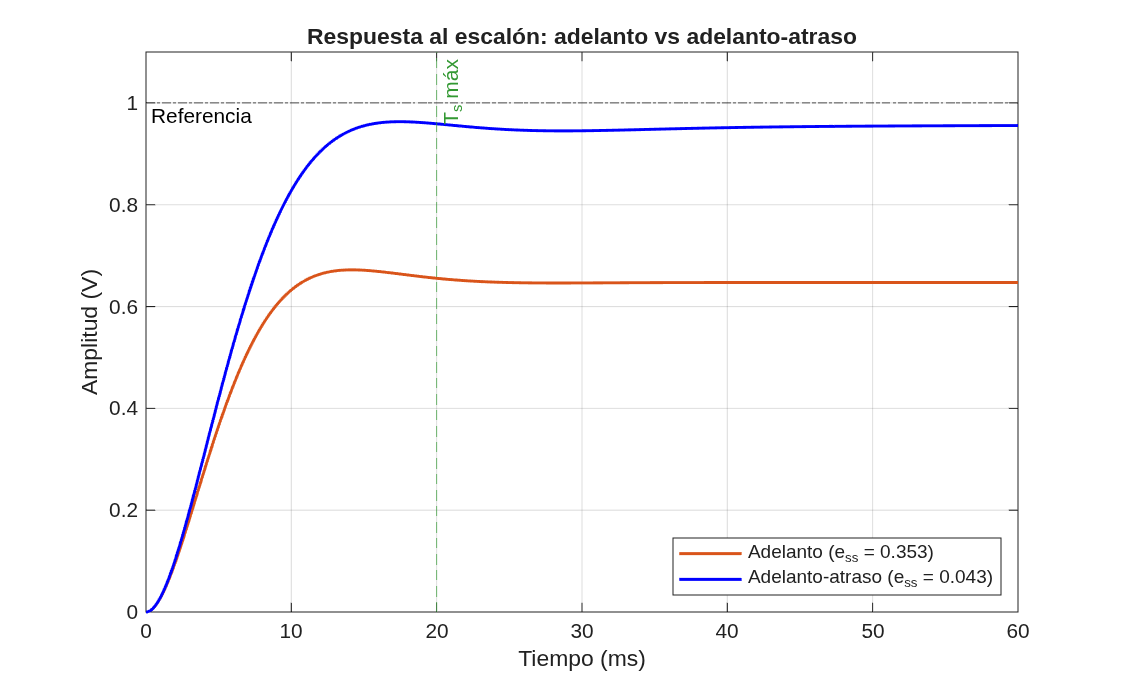
\includegraphics[width=0.78\textwidth]{figuras/punto5_comparacion.png}
    \caption{Respuesta al escalón unitario con el compensador de adelanto y con el de adelanto-atraso.}
    \label{fig:punto5_comparacion}
\end{figure}

\begin{table}[H]
    \centering
    \caption{Comparación de desempeño.}
    \vspace{2mm}
    \begin{tabular}{lccc}
        \toprule
        \textbf{Métrica} & \textbf{Requerido} & \textbf{Adelanto} & \textbf{Adelanto-atraso} \\
        \midrule
        $PO$ & $\le 5\%$ & $3{,}84\%$ & $0{,}69\%$ \\
        $T_s$ & $\le 20$ ms & $18{,}5$ ms & $13{,}5$ ms \\
        $e_{ss}$ & $\le 0{,}06$ & $0{,}353$ & $0{,}0435$ \\
        \bottomrule
    \end{tabular}
    \label{tab:comparacion}
\end{table}

\textbf{Conclusiones.}
\begin{itemize}
    \item \textbf{Adelanto:} ubica los polos dominantes en la zona que cumple $PO$ y $T_s$. Es la etapa pensada para el transitorio. No alcanza para el error, porque subir $K_p$ solo con el adelanto exige una ganancia $K_a$ que satura los amplificadores.
    \item \textbf{Atraso:} multiplica $K_p$ por $\alpha = 12$ y lleva el error de $0{,}353$ a $0{,}0435$. Como su ganancia en alta frecuencia es aproximadamente 1, el inicio de ambas respuestas es casi igual (primeros $\approx 4$ ms de la Figura~\ref{fig:punto5_comparacion}); la diferencia aparece a medida que actúa la ganancia de baja frecuencia.
    \item \textbf{Efecto del atraso sobre el transitorio:} con el cero y el polo muy cerca del origen el atraso casi no mueve los polos dominantes, pero agrega una cola lenta que hace que no se cumpla $T_s$. Ubicando $z_a = 85$ el polo de lazo cerrado asociado es rápido ($-78{,}4$); los polos complejos se mueven algo, pero el resultado final tiene menos $PO$ y menor $T_s$ que con el adelanto solo.
\end{itemize}
Con el controlador adelanto-atraso se cumplen las tres especificaciones.

\end{document}
